
\subsection{VM}

These three pieces have been completed thus far, we discuss future work in Section
\ref{sec:future}. I plan to submit the entire work to SysML 2020, in early September.


\section{Introduction}
\label{sec:Relay-intro}

As deep learning-based applications have become ubiquitous, so have systems for optimizing, executing, and deploying such applications. A number of systems research projects focus on enhancing the performance of a subset of pre-trained models produced by deep learning (DL) researchers~\citep{Dahl2011taslp, yu2011improved, han2016isca, NIPS2016johnson}.
Specifically, these models represented as static data flow graphs where the sizes of each input and output (i.e. tensors or $n$-dimensional arrays) are known a priori, ensuring the execution path remains unchanged on every invocation.
We refer to models with this static nature as \emph{static models}.
Continued advances in neural networks, especially those in natural language processing, have introduced new dynamism in models, such as control flow \citep{lstm, language_model}, dynamic data structures \citep{tree_lstm, graph_lstm}, and dynamic shapes \citep{devlin2018bert}. We refer to models exhibiting these behaviors as {\em dynamic models}.

As dynamic models mature and continue to move from research to production, it calls for an efficient and cross-platform inference system.
This poses new challenges for deep learning practitioners, as dynamic models introduce input-dependent graph topology, breaking existing system assumptions and invalidating optimizations designed for purely static data flow graphs.
% Dynamic models require an inference system to effectively and efficiently execute across various hardware platforms.
However, no existing solutions fulfill these requirements.

Many existing approaches to dynamic model optimization apply or extend existing deep learning frameworks~\citep{xu2018cavs, gao2018low, yu2018dynamic, jeong2018improving, jeong2019janus, dynet, tf_fold}.
However, deep learning frameworks optimized for training can be limiting in model inference settings due to their rich feature set. In order to realize these features frameworks are often monolithic, large, and non-portable.
%Existing work which builds on frameworks extends the programming model either via sophisticated additions~\citep{yu2018dynamic} or significant runtime overhead~\citep{tf_fold, jeong2019janus}.
%Other work~\citep{xu2018cavs, gao2018low, tf_fold} which is focused on optimizing specific types of models is often hard to generalize to new models, or generalize over all models.
Moreover, approaches which inherit from frameworks rely on third-party kernel libraries such as OpenBLAS~\citep{xianyi2014openblas}, cuDNN~\citep{cudnn}, and MKL-DNN~\citep{mkldnn} to achieve competitive performance. These libraries expose a fixed set of operators for the corresponding hardware, compromising the portability of dynamic models which require a large number of operators with varying data types and shapes. Designing a new interface independent of existing frameworks provides a clean programming model but often at the cost of performance, due to dynamic interpretation of the model~\citep{dynet}.

An alternative approach which has generated significant interest in both academia and industry is the end-to-end optimization of neural networks using deep learning compilers, such as XLA \citep{xla}, Glow \citep{glow}, TVM \citep{tvm_osdi18}, and MLIR \citep{lattner2020mlir}.
Deep learning compilers differ from traditional deep learning frameworks by separating execution into a compilation, and runtime phase. The compilation phase enables whole-model optimization at the graph level, and workload specific kernel code-generation for multiple hardware platforms.

However, deep learning compilers have been primarily restricted to static models due to lack of support for dynamism.
Specifically, in order to compile and execute the dynamic models, a system requires an intermediate representation (IR) which can statically represent dynamic constructs, a code generator
which can generate kernels for dynamically varying data shapes, and a runtime to handle the dynamic execution and kernel dispatch accordingly.
In addition, dynamic-specific optimizations, such as dynamic memory planning, the process of statically optimizing dynamic allocations, are necessary to achieve desirable performance.
None of these features exist in the current deep learning compilers.

To this end, we present Relay, a high-performance and portable system for compiling, optimizing and executing dynamic neural networks on multiple platforms.
To the best of our knowledge, this is the first attempt to systematically handle dynamic models from a compiler perspective.
First, we introduce type system extensions to handle data with unknown dimension, which is common in dynamic models, by performing type checking and inference for shapes with {\em Any}.
Second, we devise several optimizations specific to dynamic models, including dynamic shape-aware code generation, memory planning, and device placement.
Third, we propose a virtual machine (VM)-based runtime that contains tensor-level operations, enabling the exploration of new runtime and compiler optimizations as well as
being portable, light-weight, and most importantly, able to execute dynamic models.
Experimental results on LSTM~\citep{lstm}, Tree-LSTM~\citep{tree_lstm} and BERT~\citep{devlin2018bert} show that Relay~lowers the latency by 1.05$\times$ to 19.9$\times$ compared to the best solution whichever on mainstream hardware platforms both in the cloud (Intel CPUs and Nvidia GPUs) and at the edge (ARM CPUs).
%achieves lowest latency over the state-of-the-art solutions and has up to 20.3$\times$ performance speedup on mainstream hardware platforms both in the cloud (Intel CPUs and Nvidia GPUs) and at the edge (ARM CPUs).

In summary, this paper makes the following three core contributions:
\begin{itemize}
    \item Proposes and builds an end-to-end system for efficient dynamic model inference across multiple hardware platforms, including an empirical study to benchmark the results;
    \item Devises several compilation and optimization techniques,
    %for dynamic models,
    including a dynamic type system, a memory planning pass, and heterogeneous device placement mechanism to place computation and data, and a symbolic kernel code generation and shape-based dispatch algorithm;
    \item Designs and implements tensor based abstract machine with a hardware-independent instruction set to efficiently and flexibly execute dynamic models across platforms.
\end{itemize}

The rest of the paper is organized as follows. \autoref{sec:background} reviews the background of dynamic models from the system perspective and \autoref{sec:overview} gives the overview of Relay.
\autoref{sec:compliation} presents the design and implementation of the compilation flow of Relay, followed by VM-based runtime in \autoref{sec:runtime}. \autoref{sec:eval} provides the evaluation results using various models on different hardware platforms.
\autoref{sec:relwk} covers related work, and \autoref{sec:conclusion} concludes the paper.

%%%%%%%%%%%%%%%%%%%%%%%%%%%%%%%%%%%%%%%%%%%%% GRAVEYARD

%However, the dynamic nature of these models introduces input-dependent graph topology, breaking existing system assumptions.
%For example, the topology of Tree-LSTM model~\citep{tree_lstm} may change from sentence to sentence depending on its length and structure.
%The input-dependent nature of execution poses new challenges for applying existing inference optimizations to dynamic models.
%Optimizations designed for purely static data flow graphs fail to fully capture model behavior at compile-time.
%Traditionally, researchers modify models by applying workarounds to remove dynamism such as padding to maximum sequence length in order to efficiently execute. However, this may introduce unnecessary computation overhead, and is unable to handle all dynamic cases.

%Deep learning frameworks~\citep{tensorflow, mxnet, pytorch} that are optimized for

%their characteristics significantly simplify their optimization in machine learning frameworks~\citep{tensorflow,mxnet,pytorch} and compilers~\citep{tvm_osdi18,xla,glow}.

%have the following limitations and drawbacks when facing the dynamic model inference scenarios. First, the strength of deep learning frameworks is their rich functionality and optimizations for training and distribution, but often the design choices which optimize for training or distribution introduce challenges for deploying on a variety of platforms.Second, these approaches focus on handling the dynamism of models in the presence of the framework, while purely relying on the framework, and fundamentally, third-party libraries such as OpenBLAS~\citep{xianyi2014openblas}, cuDNN~\citep{cudnn}, and MKL-DNN~\citep{mkldnn} to achieve competitive performance. These libraries only cover a limited set of operators for the corresponding hardware, making it less flexible and portable to support dynamic model inference, which requires to execute a large number of operators with different data types and shapes on various platforms, including high-end server CPUs/GPUs and edge devices. As a result, the framework-based approaches come short in dynamic model inference with less favorable performance and infeasibility to diverse devices.

%Our approach provides three important properties lacking in existing approaches, (1) limited static optimization, (2) high execution overhead, (3) lack of portability and performance portability.
% First the current design assumptions of frameworks input and intermediate representations limit the ability to perform ahead of time optimization. For example TensorFlow's input format is high level, any all though it supports dynamic shapes, it does this via runtime overhead. Its compiler representation XLA only supports kernels which have fixed dimensions.
%when choosing to build a system on top of a framework the set of operators are limited by the underlying capabilities of the framework. For example most frameworks achieve competitive performance by redirecting their operators to carefully hand-crafted and well-tuned kernel libraries that target a few specific hardware architectures with fixed shape and type configurations. These third-party libraries, e.g. OpenBLAS~\citep{xianyi2014openblas}, cuDNN~\citep{cudnn}, and MKL-DNN~\citep{mkldnn}, only contain a limited set of computation-intensive operators for a given hardware platform. These limitations make it challenging to provide simple portability for dynamic models, let alone portable, state-of-the-art performance. As a result, many framework-based approaches have to confine themselves to supporting of a quite limited set of dynamic models for inference, and even when they do execute the performance can be underwhelming.

% \mli{general comments after reading this paper and review feedback. \begin{enumerate}
%     \item should highlight the difference between DL framework and DL compiler, focus on DLC's advantages such as portability, light-weight and performance.
%     \item mention that dynamic NNs are getting popular, while DLC can not deploy these models. This paper will bridge this gap.
%     \item make the system design general, such as these are necessary components to extend any static DLC. By this way we can 1) avoid the feeling that it's just a TVM extension, that will not be accepted by OSDI. 2) make it easy to read so readers don't need to learn TVM and Relay's details
%     \item The design decision of the VM is not straightforward, need to explain why we want to do it. Readers may feel it's an overkill for dynamic NN.
%     \item the performance speedup seems magic. Need to explain the reason which component make it fast
% \end{enumerate}}

% \mycomment{Talk about what are some of techniques to solve the problem and what we do...}
% \mycomment{Meanwhile, we may also want to talk about the difference between our technique and the
%           traditional compiler techniques. Memory management? Granularity of instructions?}

%\item \textbf{Optimization.} Deep learning compilers feature a host of standard compiler optimizations and deep learning specific ones at both graph-level and tensor-level. Most optimizations become non-trivial when dynamism comes into play. Memory planning is among such cases. In dynamic models, as different invocations may go through different paths that need different amounts of memory, we cannot pre-allocate memory as for static models. Furthermore, the shape of input tensors may vary depending on the provided data, i.e. the length of sentences for Tree-LSTM models. Thus, the memory optimization schemes that have worked well for static models are inapplicable to dynamic models.
%For example, operator fusion attempts to combine multiple consecutive operators into a single kernel to eliminate intermediate results, hence reducing costly back-and-forth memory loads and stores. This optimization has been implemented in a variety of deep learning compilers since the input of every operator is known before optimization. However, operator fusion across control flow inevitably complicates the fusion rules as the \texttt{if} and \texttt{else} branches may involve operators that require totally different fusion strategies.

 %Static behavior is most commonly found in image classification models, e.g., VGG~\citep{simonyan2014very}, MobileNet~\citep{howard2017mobilenets}, and ResNet~\citep{he2016deep}.
%For example, memory could be allocated before runtime and schedules could be confined to a relatively small set of parameters for each operation as the execution path is fixed for arbitrary input in the static scenario.

%primarily come from deep learning frameworks~\citep{tensorflow, mxnet, pytorch} and runtime systems~\citep{xu2018cavs, gao2018low}.
%For example, Tensorflow Fold \citep{tensorflowfold}

%%%%%%%%%%%%%%%%%%%%%%%%%%%%%%%%%%%%%%%%%%%
% old intro

% There are two clear levels to support full dynamism, dynamism introduced by the frontend language
% such as found in PyTorch and other expressive dynamic neural network frameworks. The second level of
% dynamism is innate to models, take for example a model which dynamically produces the inputs for an
% inner RNN.

% Frameworks such as PyTorch, and JAX have begun to address the first challenge by employing
% techniques from JIT compilation to find traces of user programs with stable properties (e.g., tensor
% shapes). After obtaining a stable trace the framework must produce an efficient implementation for
% the static fragment. Even if we eliminate behaviors like conditionally construction of the model
% based on whether it is executed in training or inference mode, true dynamism remains. For example
% BERT uses dynamic behavior which generates runtime dependent sized tensors. TODO CHECK THIS.

% Existing state-of-the-art optimizing compilers for deep learning provide limited support for
% efficiently compiling these type of operations. In particular the ability to quickly prototype new
% execution or compilation strategies is challenging.

% In this work we introduce Relay an extension to TVM's Relay IR which provides efficient
% compilation and execution of neural networks using data structures, control-flow, closures and
% dynamically sized tensors.

% Old contributions:
% \begin{itemize}
%     \item An extension to the type system of Relay to support dynamic dimensions.
%     \item A new efficient runtime system and virtual machine for Relay programs.
%     \item A framework for exploring code generation strategies.
%     \item A set of optimizations to improve code generation.
% \end{itemize}

\section{A System Perspective to Dynamism}
\label{sec:Relay-background}

%This section briefly discusses two representative classes of DL models: static models and dynamic models. We also explains the challenges in performing models inference for dynamic models which motivates the design of Relay.

Dynamism is now common in state-of-the-art deep learning models in various forms, i.e. control flow, data-dependent model architecture, and variable data shapes imposed by dynamic batch size and/or input length.
In the presence of these features, it becomes impossible to pre-compute certain program properties ahead of time, hence only a limited subset of optimizations available for static models can be directly reused.
In this section, we first review the existing systems to support dynamism, followed by the discussion of supporting dynamic models using deep learning compilation techniques. Based on the observation, we propose our system Relay and give an overview of it.

\subsection{Existing systems}
\label{sec:background:existing}
Researchers working on dynamic models typically use flexible deep learning frameworks to build proof of concept models, and then attempt to optimize the model using the builtin capabilities of the framework when deploying at scale.

Deep learning frameworks describe the model in either an imperative (define-by-run) or symbolic (define-then-run) fashion.
Imperative frameworks, such as DyNet~\citep{dynet} and PyTorch~\citep{pytorch}, although user friendly and flexible, may reduce performance due to eagerly executing each computation in isolation.
Both DyNet and PyTorch support executing compute-intensive operators by reusing high-performance implementations from vendor libraries, however, the inherent nature of imperative execution substantially limits optimization, i.e. no operator fusion and batching.
In addition each execution path requires the creation of a path specialized static data flow graph introducing overhead in dynamic cases, which can sometimes be unacceptable for particular application.

Not only do frameworks rely on vendor provided libraries, but many are written in a combination of multiple programming languages such as C++ and Python. The inclusion of platform specific libraries and/or arbitrary Python program fragments limits deployment and retargeting.
Platforms such as resource limited edge or embedded devices do not support these libraries and/or languages limiting these solutions from executing on some platforms without serious re-engineering, leading to solutions such as TensorFlow Lite.
Imperative programs are extremely effective at helping researchers prototype and test preliminary ideas, but not an ideal or systematic solution to deploying dynamic models at scale.

Alternatively, other deep learning frameworks use a symbolic approach, in which a user specifies the program as a data structure which can later be optimized, deployed, and executed. Frameworks in this style such as TensorFlow and MXNet already have introduced support for dynamism, such as control flow and dynamic batching~\citep{yu2018dynamic, tf_fold, mxnet-control}. Although these make it possible to use dynamic features, the extensions add complexity to an already complex programming model, and are often less integrated into the framework, requiring users to use a sophisticated modified programming model when defining dynamic models.

In addition, in some cases, it is possible to reduce the dynamic model to a static one. For example, in RNN models with variable input length, a maximal input length can be used to statically unroll the network, and padding applied to the inputs in order to directly adopt optimizations performed on static models~\citep{zhang2018deepcpu}. However, transforming a dynamic model into a static one for optimization is inflexible and only works for a subset of dynamic models. Programmability and flexibility aside, the above solutions inherit the cumbersome codebase of the deep learning frameworks which have poor portability to multiple platforms, especially edge devices. From a systems perspective, they are too heavy-weight to be adopted in these cases.

In order to enjoy the flexible description of dynamic models provided by high-level frameworks and the performance advantages of ahead of time optimization, prior work like Janus~\citep{jeong2019janus} attempted to bridge these two programming models for dynamic models.
Janus was implemented as an extension to TensorFlow which parses the model defined in TF Eager and use speculative execution to eliminate control flow constructs within the model.
Although this solution provides good performance in a subset of cases, it suffers from performance loss when speculative assumption is violated.
%\yida{@Haichen, we may also discuss the usage of ? here. Or we can defer the discussion of ? to section 3.}
Also, as it is still based on the framework, this solution inherits the drawbacks of poor portability.

Specific runtime systems were recently proposed to handle dynamic models~\citep{xu2018cavs, gao2018low}. These systems are designed to address system-level issues that plague framework-based approaches, e.g., large overhead introduced by data flow graph construction.
However, other issues, such as software dependencies, remain, which makes these runtime systems not standalone, but a customized component of a larger deep learning framework.

\subsection{Limitation of Deep Learning Compilers}
\label{sec:background:dlc}
As discussed in~\ref{sec:background:existing}, existing solutions to dynamic models have various limitations, the most pressing of which is the lack of portability and cross-platform support.
A generic system which handles dynamic models for efficient inference is missing.
Conceptually, this system should handle all dynamic models, provide portable performance across multiple platforms, and execute everywhere by virtue of being light-weight and dependency-free.
With these goals in mind, deep learning compilers are a promising direction to explore, as these techniques aim to perform end-to-end optimization on models that can run with minimal memory footprint over multiple platforms.


% \begin{figure}[t]
%   \centering
%   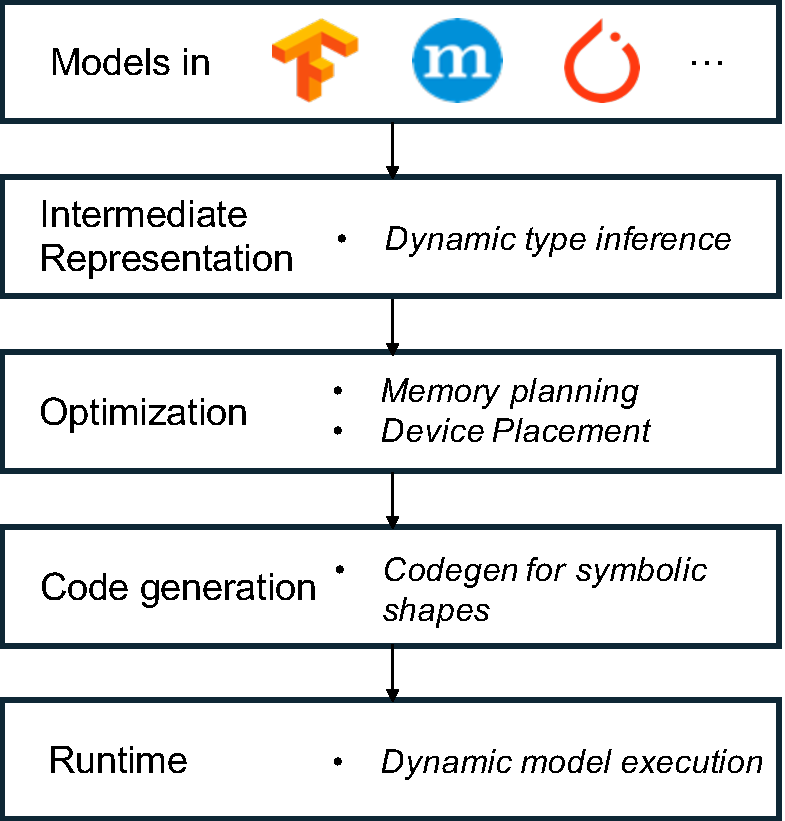
\includegraphics[width=.7\linewidth]{figs/dlc.pdf}
%   \captionof{figure}{
%   %\protect\yida{Can delete this figure if running out of space.}
%   A generic deep learning compiler workflow in multiple stages. Existing deep learning compilers are unable to process dynamic models due to lacking of the functionalities listed in each stage.}
%   \label{fig:dlc}
% \end{figure}

However, current deep learning compilers are not able to process dynamic models due to missing the following dynamism-specific features.% in the \emph{type system}, \emph{codegen}, and \emph{runtime}, along with dynamism-oriented optimizations such as \emph{memory planning} and \textit{heterogeneous device placement}.

\begin{itemize}
\item \textbf{An IR for representing dynamism.} Performing data type and shape inference on static models is straightforward as both the data type and shape of each operator are known during declaration and remain unchanged during runtime. However, the shape of an input tensor may vary wildly across different input samples in a dynamic model. The emergence of control flow constructs further complicates this problem as different execution paths can emit substantially different data. A fully static IR, hence, is inadequate to cope with the dynamic characteristics of these models.

\item \textbf{A set of dynamic-oriented optimizations.} Existing deep learning compilers, e.g. TVM \citep{tvm_osdi18} and Glow \citep{glow}, expect static input for each optimization. The memory size of each tensor is pre-allocated and their live cycles are determined using a dedicated optimization pass. They also ensure the homogeneous execution of the entire model because all kernels are executed on the same device with no data transfer between the host and device after a kernel is launched. However, these optimizations may completely break when dynamism appears. Now different execution path possibly requires different amount of memory and the sizes are not available before runtime. Certain simple IR nodes may also be introduced to help runtime type inference and memory allocation. The operations in these nodes are intrinsically more CPU friendly, which would lead to the serious performance problem if not placed on the correct device.

\item \textbf{A symbolic kernel code generator.}
Code generation (codegen) is responsible for generating high-performance executable kernels for operators. Recent research \citep{tvm_osdi18, glow, chen2018learning, zheng2020flextensor, adams2019learning} has achieved impressive results in kernel performance with static shapes on multiple backends.
Nonetheless, challenges in codegen with symbolic shapes remain unexplored.
After applying the same set of loop optimization, kernels generated with symbolic shapes could still perform bad if the loop boundary is not handled properly.
Meanwhile, kernel tuning under symbolic shape settings become more challenging as the search space grows exponentially.

%\yida{@Haichen, please revise this part accordingly. I feel that we should talk about about symbolic. And perhaps make it shorter, comparable with the other two points}
% The same operator (e.g. convolution) with different data shapes may require different kernels with different execution schedules to obtain preferable performance. There is no ``one-size-fits-all'' kernel and/or schedule that delivers consistently ``the-best'' performance across invocations with vastly different data shapes in a dynamic model. Instead, it requires the code generator to take the varied shapes into consideration and possibly generate a family of specialized kernels to maximize the performance of a dynamic operation. In addition, some common operators are well-optimized on specific platforms (e.g. MKL-DNN for Intel CPU and CuBlas for Nvidia GPU), and the code generator should be able to select kernels from third-party libraries if they will achieve the best end-to-end performance.

\item \textbf{A light-weight and cross-platform runtime.} For efficiency purpose, the runtime of static models could be simply designed a sequential executor that traverses the input data flow graph in the topological order and invokes operators sequentially. However, the execution path of dynamic models can only be determined at runtime and the kernels for certain operators must be dispatched according to the data shape determined at runtime, making a simple graph-style runtime insufficient.
\end{itemize}

Figure~\ref{fig:dlc} summarizes a generic deep learning compiler workflow in multiple stages, with the missing parts to supporting dynamism listed in each stage.  %\zhicomment{Figure needs to be updated, add heterogeneous device placement to optimization}.

% ------------------------------------------


% \subsubsection{Memory pass}

% \subsubsection{Symbolic code generation}

% \subsubsection{VM overhead}
% \label{sec:eval:overhead}
% Finally, we compared the performance of model inference for static neural networks using Relay with unmodified TVM. TVM is known to be efficient in processing CNN models on various hardware platforms~\citep{tvm_osdi18, liu2019optimizing}. Relay extended TVM to support dynamism while inheriting the optimizations original TVM has. Relay's VM-based runtime was designed to be generic enough to handle static model inference as well. Therefore, comparing between Relay and the original TVM on static model inference should indicate how much overhead Relay introduces while introducing dynamic support.

% \autoref{fig:static-performance} and \autoref{fig:memory-overhead} show the latency and memory footprint comparison between Relay and original TVM on different static CNN models. The models were optimized via the TVM pipeline in both systems. The difference is that Relay uses its VM-based runtime while TVM uses its original graph runtime. From the figure we can tell that Relay's VM-based runtime adds minimal overhead compared to TVM's original runtime, by adding up to 13\% more execution time and 8\% more memory footprint. Also, \autoref{fig:memory-overhead} further testifies that our memory planning optimization reduces the memory usage on static model inference as well.

% We have evidence that this overhead is due to missing micro-optimizations, and not inherent to our approach, and should be erased over time.

% \begin{figure}
% \centering
% \input{figs/static_perf}
% \caption{Latency comparison between Relay and TVM on static model inference. The latency was tested for both systems on Intel CPUs, Nvidia GPUs and ARM CPUs by setting batch size=1. The latency of TVM on those platforms was normalized to 1, the lower the better.}
% \label{fig:static-performance}
% \end{figure}

% \begin{figure}
% \centering
% \input{figs/memory}
% \caption{Memory usage comparison between Relay and TVM on static models. Relay was done with and without optimization on memory planning. The results were obtained on Intel CPUs. Nvidia GPUs and ARM CPUs would lead to the identical results. The amount of memory used by TVM was normalized to 1, the lower the better.}
% \label{fig:memory-overhead}
% \end{figure}

%%%%%%%%%%%%%%%%%%%%%%%%%%%%%%%%%%%%%%%%%%%%%%%%%%%%%%%%%%%%%%%%555

%\vspace{-1em}
\subsection{Memory Planning}
\label{sec:compliation:memory}

Deep learning workloads are dominated by two key components,
    compute-intensive kernels and memory allocation.
Many deep learning compilers use a form of static memory planning
    coalesces memory into contiguous chunks and minimize allocations.
For devices such as GPUs these optimizations are essential for
    reducing memory fragmentation and ensuring allocation does not hamper kernel performance.
Existing deep learning compiler IRs hide memory allocation behind a
    functional interface, where each operator implicitly allocates their output storage.
Then before execution, the system performs static-memory planning on the data
    flow graph enabling efficient pre-allocation of the required output buffers.
Due to this ``out-of-band'' nature of memory allocation,
    it is challenging to customize, modify, or compose memory optimizations with other passes.
For example, if one needs to adjust memory allocation for heterogeneous execution,
    modifications to the runtime system are required.
TVM's graph runtime is one such example of static memory planning.
Due to the coarse-grained memory semantics of deep learning models,
    it is essential that memory optimizations occur at a suitably high-level of abstraction,
    unlike traditional compilers.
Existing work provides no clear path to performing static optimization on dynamic memory
    allocation.

In order to perform what we refer to as ```dynamic memory planning'' we have extended
    TVM to transform its IR with implicit memory allocations to one with explicit
    buffer allocation and manipulation.
The key to this transformation is an inter-procedural change of calling convention,
    with each operator now taking its outputs explicitly.
The transformation makes it possible to track and optimize dynamic memory allocations in the IR.
In order to perform this optimization we have introduced four new IR constructs,
    (a) \verb|invoke_mut(op, inputs, outputs)| which takes outputs as mutable in-out arguments,
    (b) \texttt{alloc\_storage(size, alignment, device)} which allocates a region of memory of a particular size,
    (c) \texttt{alloc\_tensor(storage, offset, shape, dtype, attrs)} which allocates a tensor at a particular storage offset with a shape and data type, and
    (d) \verb|kill(tensor)| which frees a tensor before its reference count becomes zero due to exiting the frame.

We illustrate how this works with an example of transforming a single statically shaped operation such as broadcasting addition.
Note that in the below code examples \texttt{Tensor<d1, ..., dn>} is shorthand for a tensor of shape \texttt{(d1, ..., dn)} containing floating point values.

%\begin{Verbatim}[fontsize=\small]
\begin{lstlisting}
fn main() -> Tensor<10> {
  let t1, t2 : Tensor<10> = ...;
  add(t1, t2)
}
\end{lstlisting}
\vspace{-1em}
%\end{Verbatim}

Here we only must allocate a single buffer, that is, the return buffer for the addition operation.

%\begin{Verbatim}[fontsize=\small]
\begin{lstlisting}
fn main() -> Tensor<10> {
  let t1 = ...; let t2 = ...;
  let buf1 = alloc_storage(40,64,cpu);
  let out1 = alloc_tensor(buf1,0,(10),f32);
  invoke_mut(add, (t1, t2), (out1));
  out1
}
\end{lstlisting}
\vspace{-1em}
%\end{Verbatim}

The above transformation replaces the operator invocation \verb|add| to code which
first allocates an output tensor from backing storage at offset zero, and call to
\verb|invoke_mut|.
For the sake of space, we present a more complex example in the \autoref{appx:mem-plan-example}, which illustrates how to handle memory allocation when operators have dynamic shaped inputs.
The key insight is to internalize a notion of memory allocation into the IR, enabling static optimization of
both static and dynamic allocations in the presence of control and dynamic shapes.
Now that all allocations are explicit in the IR, we can provide analogous optimizations in the static
case on dynamic programs, for example we have implemented a storage coalescing pass to group storage
into a larger region which allows the multiplexing of multiple tensor allocations to a single piece of storage.
Futher optimization like liveness analysis and graph coloring algorithm can be applied to the program to reuse  the storages.
